% Copyright 2004 by Till Tantau <tantau@users.sourceforge.net>.
%
% In principle, this file can be redistributed and/or modified under
% the terms of the GNU Public License, version 2.
%
% However, this file is supposed to be a template to be modified
% for your own needs. For this reason, if you use this file as a
% template and not specifically distribute it as part of a another
% package/program, I grant the extra permission to freely copy and
% modify this file as you see fit and even to delete this copyright
% notice. 

\documentclass{beamer}
\usepackage[normalem]{ulem}
%\usepackage{algorithmicx}
\usepackage[utf8]{inputenc} % Swedish symbols
%\usepackage{algpseudocode}
% There are many different themes available for Beamer. A comprehensive
% list with examples is given here:
% http://deic.uab.es/~iblanes/beamer_gallery/index_by_theme.html
% You can uncomment the themes below if you would like to use a different
% one:
\usepackage{verbatim}
\usepackage{listings}
\usepackage{color}
\usepackage{xcolor}
\usepackage{tikz}
\usepackage{qtree}
\usepackage{caption}

\definecolor{dkgreen}{rgb}{0,0.6,0}
\definecolor{gray}{rgb}{0.5,0.5,0.5}
\definecolor{mauve}{rgb}{0.58,0,0.82}

\lstset{frame=tb,
  language=TeX,
  aboveskip=3mm,
  belowskip=3mm,
  showstringspaces=false,
  columns=flexible,
  basicstyle={\footnotesize\ttfamily},
  numbers=none,
  numberstyle=\tiny\color{gray},
  keywordstyle=\color{blue},
  commentstyle=\color{dkgreen},
  stringstyle=\color{mauve},
  breaklines=true,
  breakatwhitespace=true,
  tabsize=3
}

\definecolor{datagulTOP}{RGB}{251,203,19}
\definecolor{datagulSIDE}{RGB}{175,141,13}


%\usetheme{AnnArbor}
%\usetheme{Antibes}
%\usetheme{Bergen}
\usetheme{Berkeley}
%\usetheme{Berlin}
%\usetheme{Boadilla}
%\usetheme{boxes}
%\usetheme{CambridgeUS}
%\usetheme{Copenhagen}
%\usetheme{Darmstadt}
%\usetheme{default}
%\usetheme{Frankfurt}
%\usetheme{Goettingen}
%\usetheme{Hannover}
%\usetheme{Ilmenau}
%\usetheme{JuanLesPins}
%\usetheme{Luebeck}
%\usetheme{Madrid}
%\usetheme{Malmoe}
%\usetheme{Marburg}
%\usetheme{Montpellier}
%\usetheme{PaloAlto}
%\usetheme{Pittsburgh}
%\usetheme{Rochester}
%\usetheme{Singapore}
%\usetheme{Szeged}
%\usetheme{Warsaw}

%%%%%%%%


% Gives the layout colors..
\usecolortheme{wolverine}
\setbeamercolor{structure}{fg=black}
\setbeamercolor{frametitle}{bg=datagulTOP}
\setbeamercolor{sidebar}{bg=datagulSIDE}
\setbeamercolor{normal text}{bg=white, fg=black}
%\setbeamercolor{thesection}{fg=red}
%\setbeamercolor{example text}{fg=brown}

\lstset{escapeinside={<@}{@>}}
\title{\LaTeX \hspace{1 mm} Tutorial}
\subtitle{gotta TeX good.}
\author{Johan Burström}
\date{\today}
% - Either use conference name or its abbreviation.
% - Not really informative to the audience, more for people (including
%   yourself) who are reading the slides online

\newcommand{\hejsan}{something cool}

\newcommand{\fstcmd}[1][]{cmd1 #1 \sndcmd[#1]}
\newcommand{\sndcmd}[1][]{cmd2 #1}

\subject{\LaTeX}
% This is only inserted into the PDF information catalog. Can be left
% out. 

% If you have a file called "university-logo-filename.xxx", where xxx
% is a graphic format that can be processed by latex or pdflatex,
% resp., then you can add a logo as follows:

 \pgfdeclareimage[height=1.5cm]{university-logo}{ddos2.jpg}
 \logo{\pgfuseimage{university-logo}}

% Delete this, if you do not want the table of contents to pop up at
% the beginning of each subsection:
\AtBeginSection[]
{
 
  \begin{frame}<beamer>{Outline}
    \tableofcontents[currentsection]
  \end{frame}
}

\AtBeginSubsection[]
{
  \begin{frame}<beamer>{Outline}
    \tableofcontents[currentsection,currentsubsection]
  \end{frame}
}

% Let's get started
\begin{document}

\begin{frame}
  \titlepage
\end{frame}


\begin{frame}{Outline}
  \tableofcontents
  % You might wish to add the option [pausesections]
\end{frame}

% Section and subsections will appear in the presentation overview
% and table of contents.

\section{Introduction}
\subsection{Getting started}
\begin{frame}{Introduction to \LaTeX}{"How hard can it be?"}
    \begin{itemize}
        \item<1>{Go and download miktex, texmaker, texstudio, kile or some else TeX-editor}\pause
        \item{\sout{Go and download miktex, texmaker, texstudio, kile or some else TeX-editor}}
        \item{Just go to \texttt{http://www.sharelatex.com} instead}
    \end{itemize}
\end{frame}

\subsection{Sharelatex}
\begin{frame}{Share\LaTeX}{Getting started}
    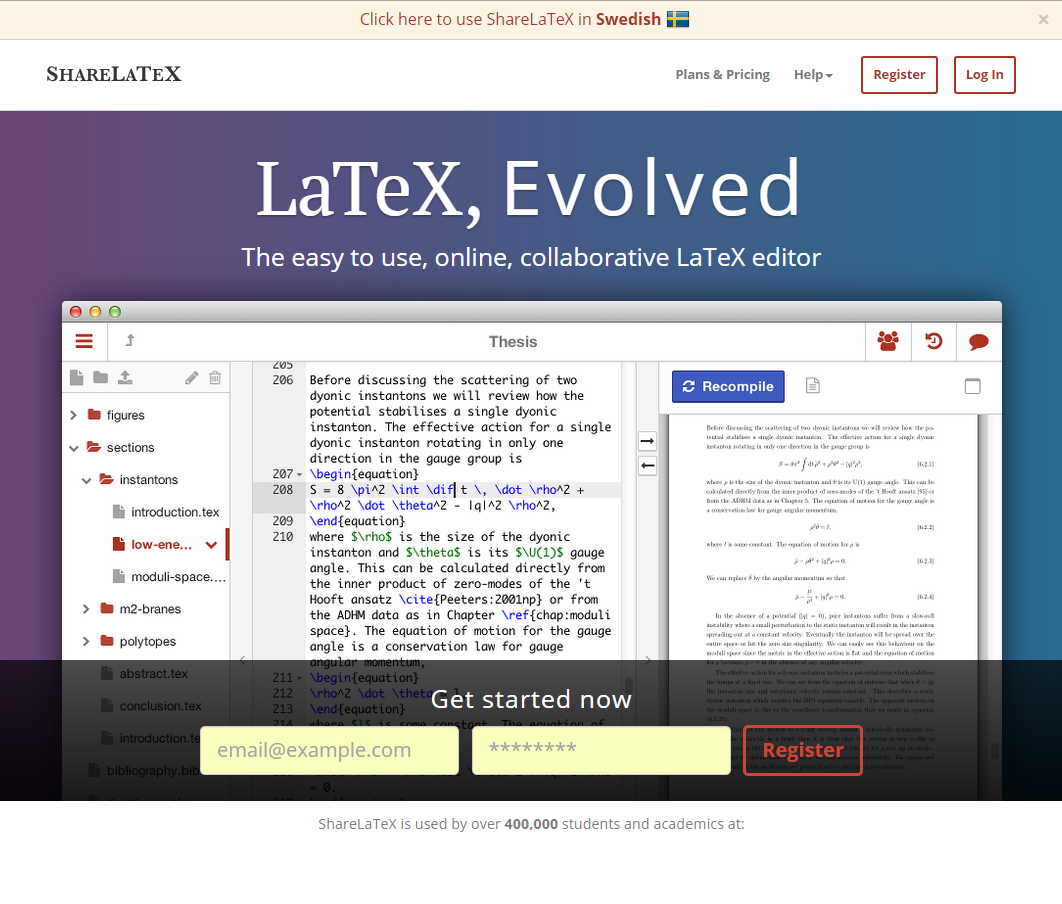
\includegraphics[width=\textwidth]{img/1-sharelatex1.png}
\end{frame}

\begin{frame}{Share\LaTeX}{Tutorial!}
    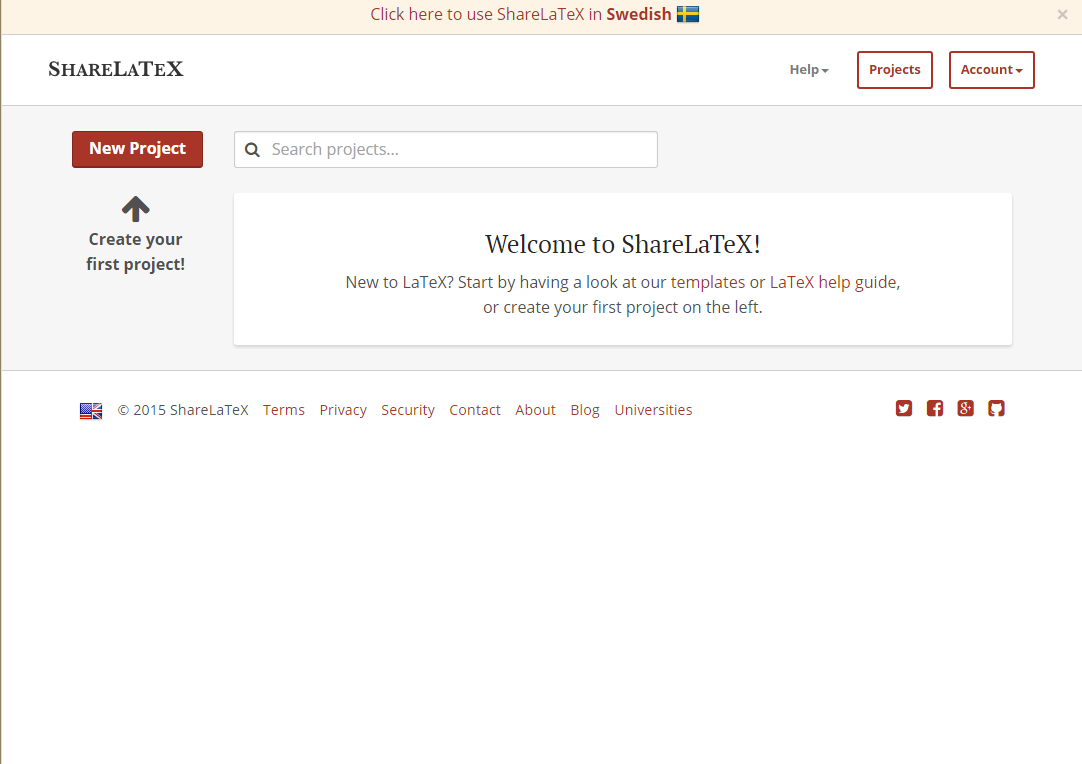
\includegraphics[width=\textwidth]{img/1-sharelatex2.png}
\end{frame}

\begin{frame}{Share\LaTeX}{Help and Templates!}
	\begin{tabular}{c c}
		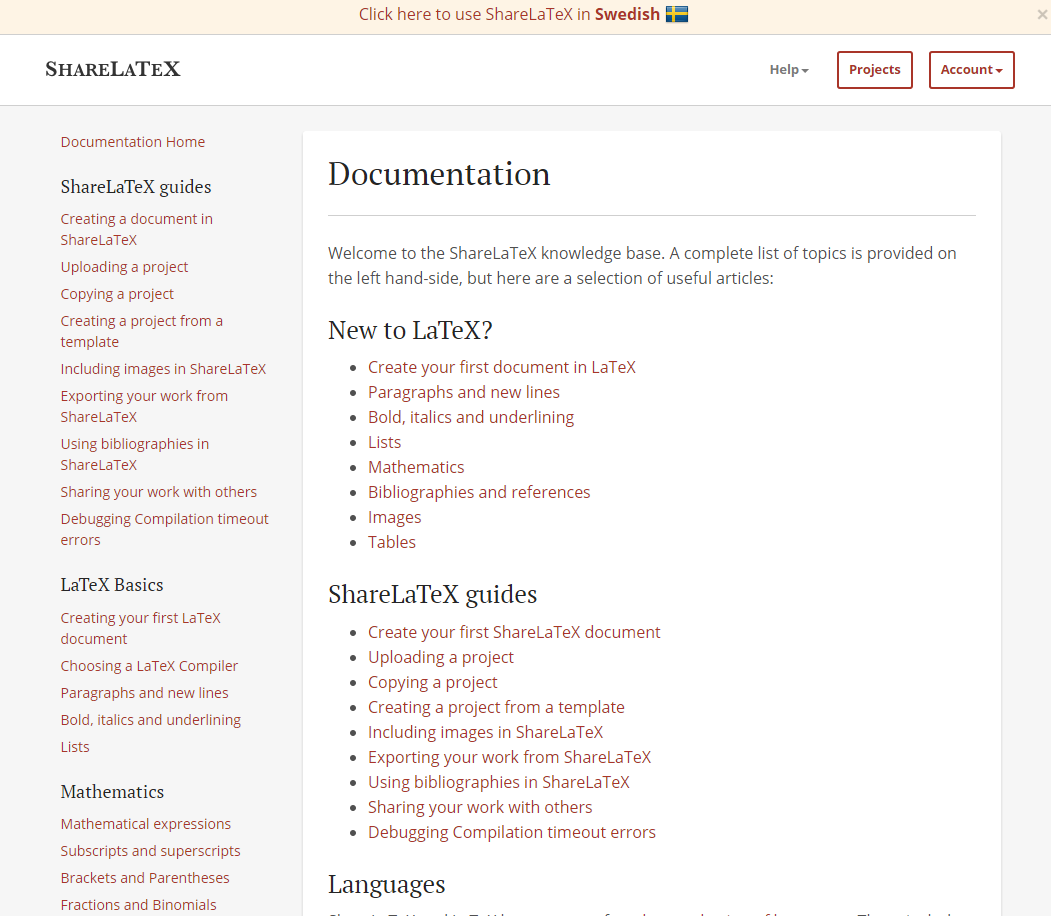
\includegraphics[width=0.5\textwidth]{img/1-sharelatex3-1.png} & 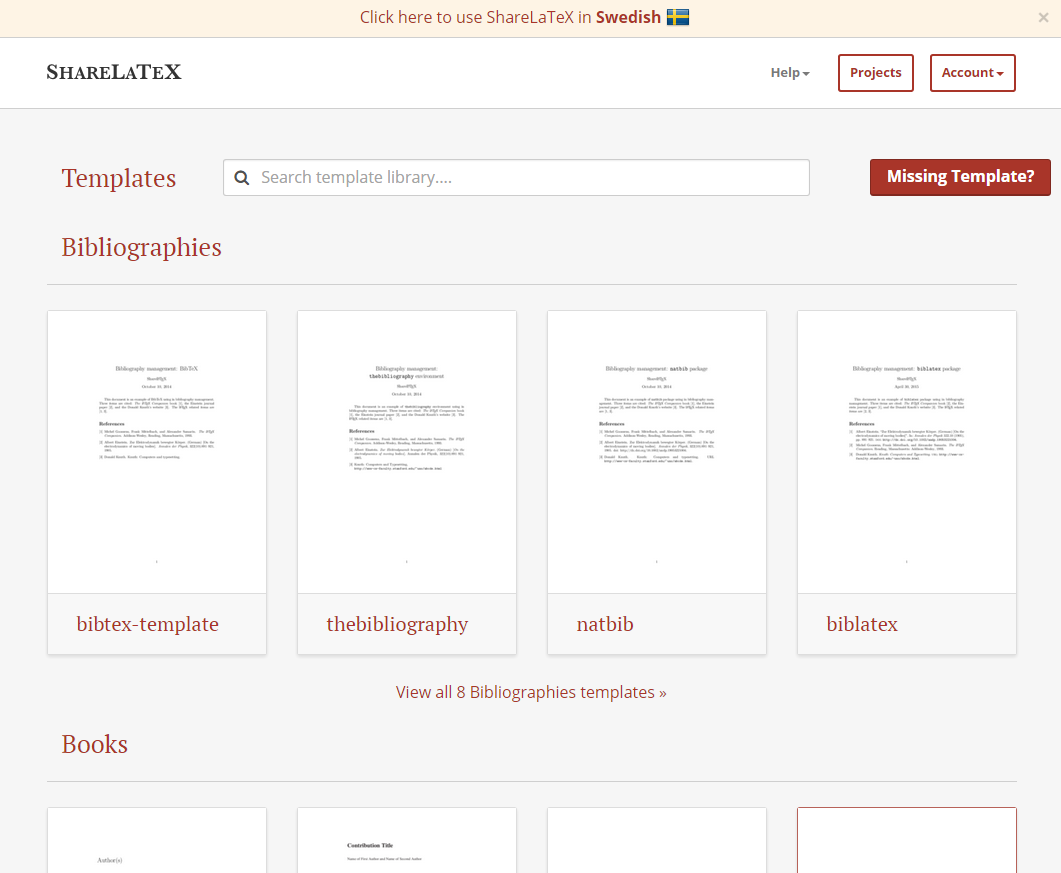
\includegraphics[width=0.5\textwidth]{img/1-sharelatex3-2.png}
	\end{tabular}
\end{frame}
\section{CV template}
% This is unique for class presentation.
\newcommand{\where}{in the facebook event.}
\begin{frame}{\LaTeX CV-template}{Can be found \where}
    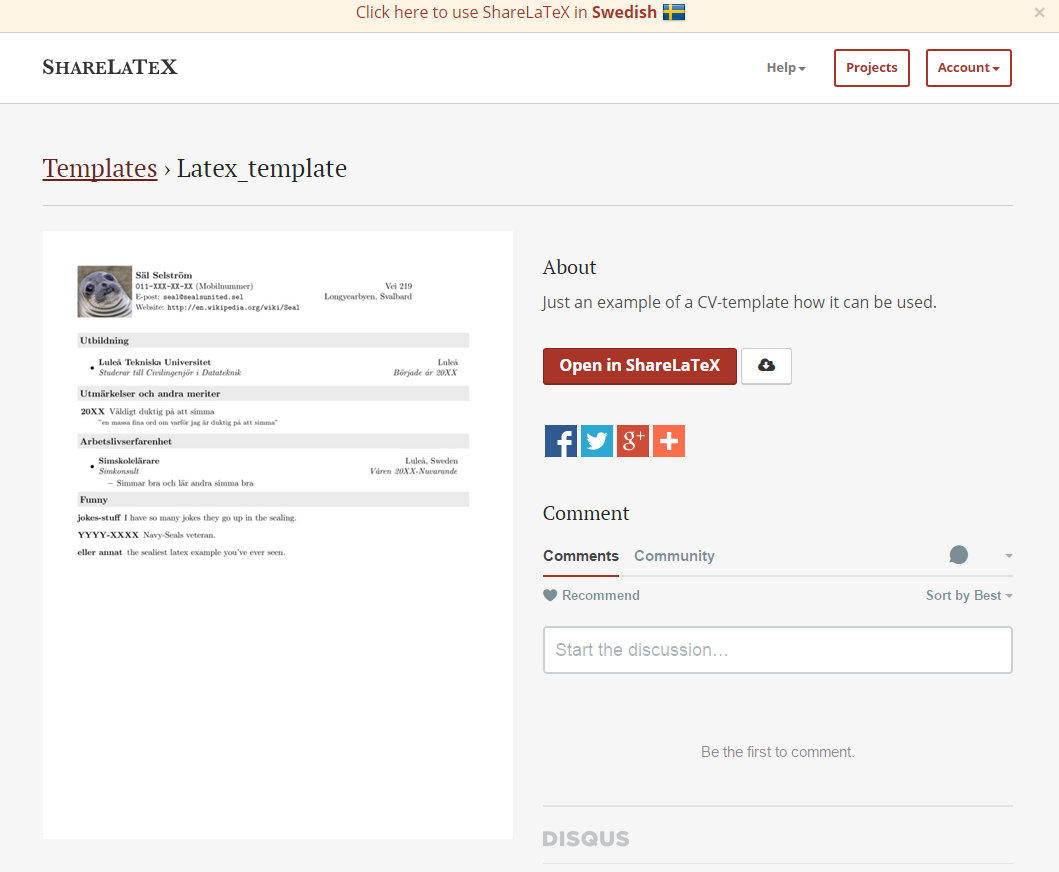
\includegraphics[width=\textwidth]{img/2-cvlatex.png}
\end{frame}

\begin{frame}{\LaTeX CV-template}{Can be found \where}
    Take some time and download the template. \\ \ \\ \ \\
    \small This link also works: \\ \ \\ \ \\
    \normalsize
    \texttt{http://tinyurl.com/ddoslatex}
\end{frame}

\begin{frame}{\LaTeX CV-template}
	Things to notice: \\ \ 
	\begin{itemize}
	\item \textbackslash newcommand
	\item \textbackslash minipage
	\end{itemize} 
\end{frame}

\subsection{Newcommand}
\begin{frame}[fragile]{Defining your own commands}
	\begin{block}{A way of defining new commands}
	\begin{lstlisting}
	\newcommand{\command}{something}
	\end{lstlisting}
		When calling \textbackslash command, we would get: 
		\begin{lstlisting}
		<@\textcolor{blue}{something}@>
		\end{lstlisting}
	\end{block}
   	\begin{block}{With arguments}
   		\begin{lstlisting}
		\newcommand{\command}[1]{something #1}
		\end{lstlisting}
		When calling \textbackslash command[seal], we would get:	
		\begin{lstlisting}
		something seal
		\end{lstlisting}
   \end{block}
\end{frame}

\begin{frame}[fragile]{Commands calling other commands}
	\begin{block}{A command calling another command}
	   	\begin{lstlisting}
		\newcommand{\fstcmd}[1][]{cmd1 #1 \sndcmd[#1]}
		\newcommand{\sndcmd}[1][]{cmd2 #1}
		\end{lstlisting}
		When calling \textbackslash fstcmd[seal], we would get: 
		\begin{lstlisting}
		<@\fstcmd[seal]@>
		\end{lstlisting}
   \end{block}
\end{frame}

\subsection{Minipage}
\begin{frame}[fragile]{A page in a page}
	\begin{block}{Acts like boxes.}
	\begin{lstlisting}
		\begin{minipage}[pos][height][contentpos]{width}
	\end{lstlisting}
   \end{block}
\end{frame}

\begin{frame}{Minipage}{Split pages?}
    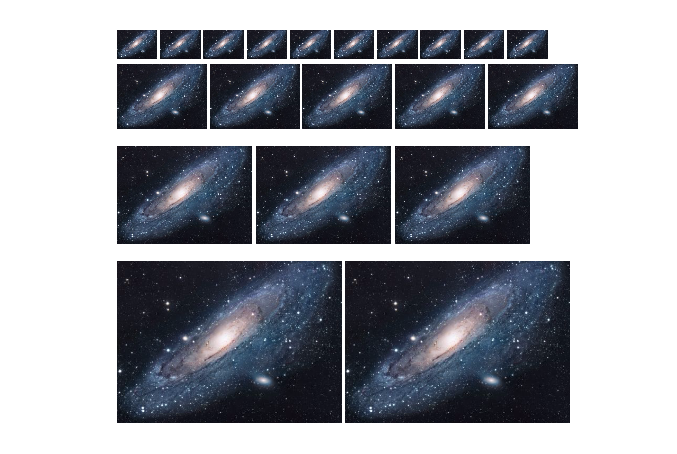
\includegraphics[width=\textwidth]{img/2-minipage.png}
\end{frame}

\begin{frame}[fragile]{Minipage - Continued}{\textbackslash begin\{minipage\}[pos][height][contentpos]\{width\}}
   more reading:
   \begin{lstlisting}
   http://en.wikibooks.org/wiki/LaTeX/Boxes#minipage_and_parbox
   http://www.sascha-frank.com/latex-minipage.html
   \end{lstlisting}
\end{frame}
\section{Protocol Template}
% This is unique for class presentation.
\begin{frame}{\LaTeX Meeting-protocol}{Can be found \where}
    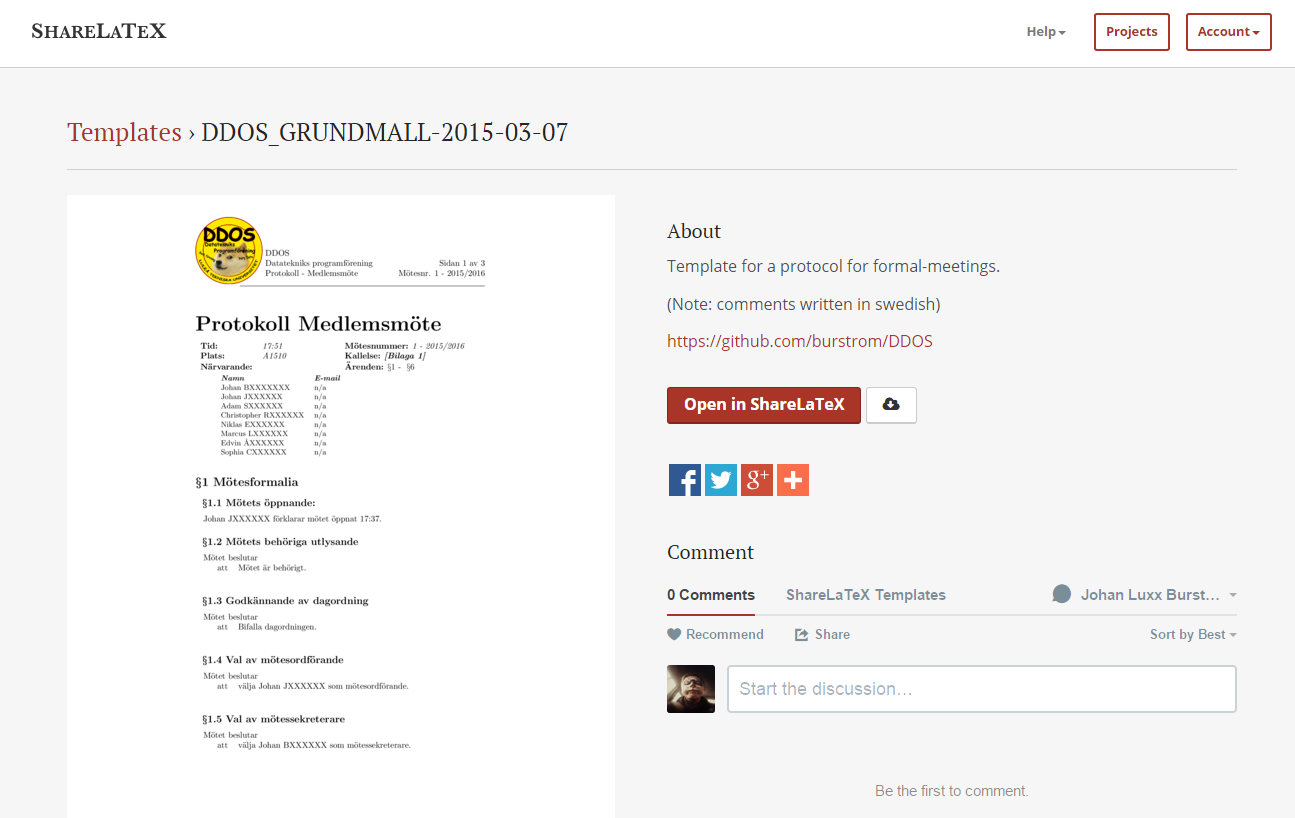
\includegraphics[width=\textwidth]{img/3-protlatex.png}
\end{frame}

\begin{frame}{\LaTeX Meeting-protocol}{Can be found \where}
    Take some time and download the template also. \\ \ \\ \ \\
    \small This link also works: \\ \ \\ \ \\
    \normalsize
    \texttt{http://tinyurl.com/ddoslatex}
\end{frame}

\begin{frame}{\LaTeX Meeting-protocol}
	Things to notice: \\ \ 
	\begin{itemize}
	\item \textbackslash newcommand
	\item \textbackslash minipage
	\end{itemize} 
\end{frame}

\subsection{Packages}
\begin{frame}[fragile]{Good packages to lookup.}
	\begin{block}{The following packages are great!}
	\begin{lstlisting}
		fancyhdr,
		pdfpages,
		calc
	\end{lstlisting}
	\end{block}
	\begin{block}{Fancyhdr}
	Gives header, margin notes, and much more.
	\textcolor{blue}{http://texdoc.net/texmf-dist/doc/latex/fancyhdr/fancyhdr.pdf}
	\end{block}
	\begin{block}{pdfpages}
	lets you include pdf-files, very useful for attachments!
	\textcolor{blue}{http://texdoc.net/texmf-dist/doc/latex/pdfpages/pdfpages.pdf}
	\end{block}	

\end{frame}
\begin{frame}[fragile]{Packages continued..}
	\begin{block}{calc}
	Adds expressions to perform arithmetic on arguments.
		Also important to use if you want to use counters!
	\textcolor{blue}{http://texdoc.net/texmf-dist/doc/latex/pdfpages/pdfpages.pdf}
	\end{block}
\end{frame}

\subsection{Counters}
\begin{frame}[fragile]{Counters can be useful for manually fixing values.}
	\begin{block}{To create a counter}
	   	\begin{lstlisting}
		\newcounter{cnter} % First initiate the counter
		\setcounter{cnter}{0} % default 0, if it's not set manually
		\end{lstlisting}
   \end{block}
   	\begin{block}{To use our counter}
	   	\begin{lstlisting}
			\thecnter % Returns the value of the counter
			\stepcounter{cnter} % increases the value
		\end{lstlisting}
   \end{block}
\end{frame}
\section{A bit more commands}
% This is unique for class presentation.

\begin{frame}{tikz package}{http://www.texample.net/tikz/examples/tag/graphs/}
\begin{minipage}[b]{0.4\textwidth}
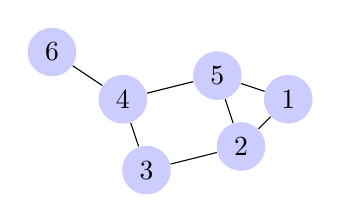
\begin{tikzpicture}
  [scale=.3,auto=left,every node/.style={circle,fill=blue!20}]
  \node (n6) at (1,10) {6};
  \node (n4) at (4,8)  {4};
  \node (n5) at (8,9)  {5};
  \node (n1) at (11,8) {1};
  \node (n2) at (9,6)  {2};
  \node (n3) at (5,5)  {3};

  \foreach \from/\to in {n6/n4,n4/n5,n5/n1,n1/n2,n2/n5,n2/n3,n3/n4}
    \draw (\from) -- (\to);

	\end{tikzpicture}
	\end{minipage}
	\begin{minipage}[b]{0.4\textwidth}
	    \begin{block}{}
	    	Very useful package for graphics and such. \\
			But this is not something I will go into detail in.
		\end{block}
	\end{minipage}
\end{frame}

\begin{frame}{More trees with qtree}{http://www.ling.upenn.edu/advice/latex/qtree/qtreenotes.pdf}
	\begin{minipage}[b]{0.4\textwidth}
	\footnotesize
		\Tree[.IP [.NP [.Det \textit{the} ]
               [.N\1 [.N \textit{package} ]]]
          [.I\1 [.I \textsc{3sg.Pres} ]
                [.VP [.V\1 [.V \textit{is} ]
                           [.AP [.Deg \textit{really} ]
                                \qroof{\textit{to use}}.CP ]]]]]
    \normalsize
	\end{minipage}
	\begin{minipage}[b]{0.4\textwidth}
	    \begin{block}{}
	    	Very useful package for graphics and such. \\
			But this is not something I will go into detail in.
		\end{block}
	\end{minipage}
\end{frame}

\begin{frame}[fragile]{Image placement - Place images anywhere?}{http://staff.www.ltu.se/~johanc/teaching.htm}
	\begin{minipage}[b]{0.4\textwidth}
	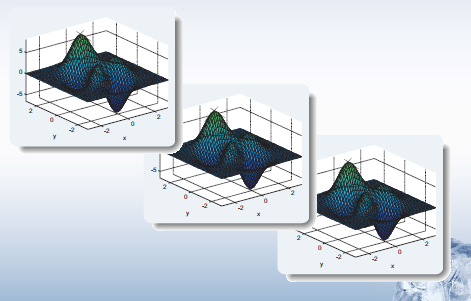
\includegraphics[width=\textwidth]{img/4-imagefloat.png}
	\end{minipage}
	\begin{minipage}[c]{\textwidth}
	    \begin{block}{}
	    	\begin{lstlisting}
				\putimageblock{.55}{.95}{.25}{peaks.pdf}
				\putimageblock{.35}{.80}{.25}{peaks.pdf}
				\putimageblock{.15}{.65}{.25}{peaks.pdf}
			\end{lstlisting}
		\end{block}
	\end{minipage}
		
\end{frame}
\section{Playaround}
\begin{frame}{Try yourself!}{\LaTeX \mbox{} is amazing}
\begin{thebibliography}{9}
	\setbeamertemplate{bibliography item}[online]
	\bibitem{A} Follow our github page, all files can be downloaded from there. \\ \ \\
	\small https://github.com/LTUDDOS/DDOS \normalsize
\end{thebibliography}	
\end{frame}

%\section{Playaround}
% This is unique for class presentation.
\begin{frame}{\LaTeX Meeting-protocol}{Can be found \where}
    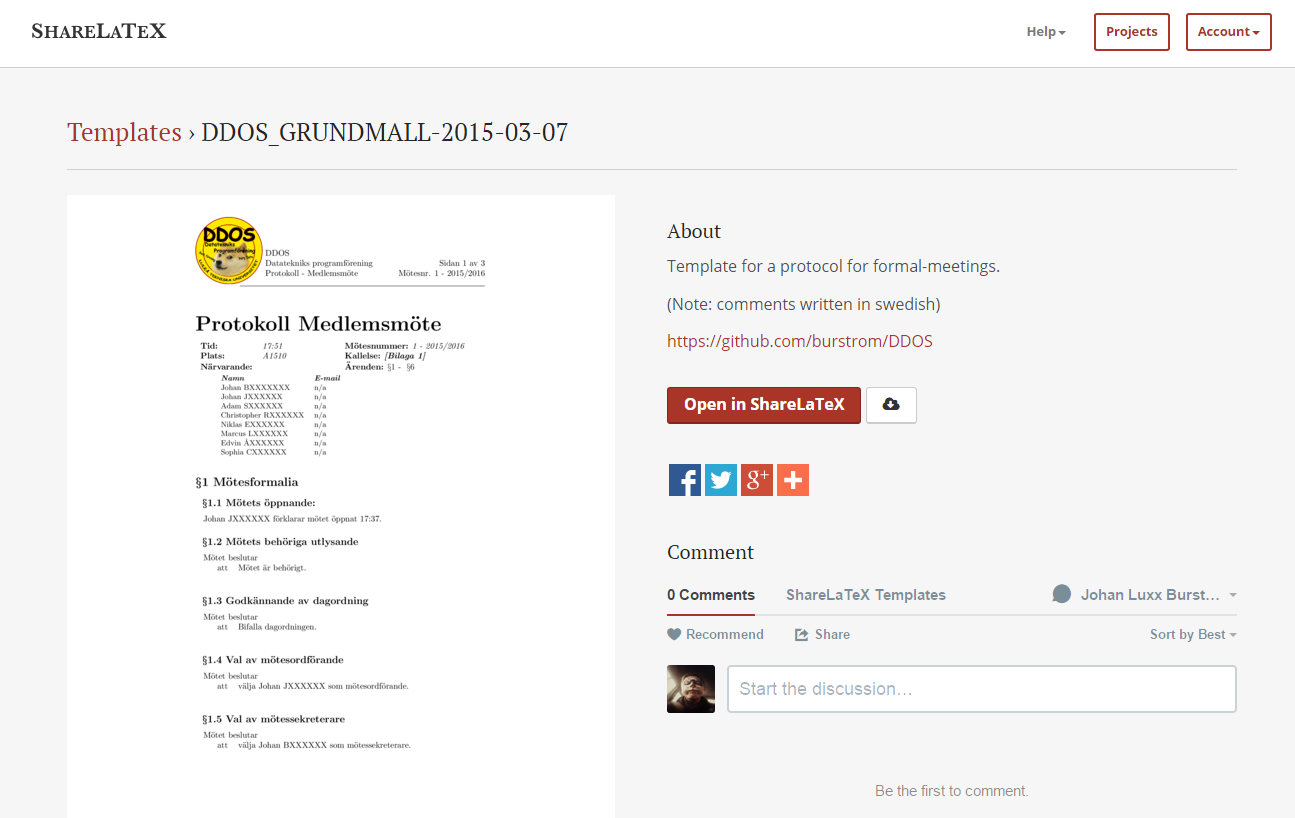
\includegraphics[width=\textwidth]{img/3-protlatex.png}
\end{frame}

\begin{frame}{\LaTeX Meeting-protocol}{Can be found \where}
    Take some time and download the template also. \\ \ \\ \ \\
    \small This link also works: \\ \ \\ \ \\
    \normalsize
    \texttt{http://tinyurl.com/ddoslatex}
\end{frame}

\begin{frame}{\LaTeX Meeting-protocol}
	Things to notice: \\ \ 
	\begin{itemize}
	\item \textbackslash newcommand
	\item \textbackslash minipage
	\end{itemize} 
\end{frame}

\subsection{Packages}
\begin{frame}[fragile]{Good packages to lookup.}
	\begin{block}{The following packages are great!}
	\begin{lstlisting}
		fancyhdr,
		pdfpages,
		calc
	\end{lstlisting}
	\end{block}
	\begin{block}{Fancyhdr}
	Gives header, margin notes, and much more.
	\textcolor{blue}{http://texdoc.net/texmf-dist/doc/latex/fancyhdr/fancyhdr.pdf}
	\end{block}
	\begin{block}{pdfpages}
	lets you include pdf-files, very useful for attachments!
	\textcolor{blue}{http://texdoc.net/texmf-dist/doc/latex/pdfpages/pdfpages.pdf}
	\end{block}	

\end{frame}
\begin{frame}[fragile]{Packages continued..}
	\begin{block}{calc}
	Adds expressions to perform arithmetic on arguments.
		Also important to use if you want to use counters!
	\textcolor{blue}{http://texdoc.net/texmf-dist/doc/latex/pdfpages/pdfpages.pdf}
	\end{block}
\end{frame}

\subsection{Counters}
\begin{frame}[fragile]{Counters can be useful for manually fixing values.}
	\begin{block}{To create a counter}
	   	\begin{lstlisting}
		\newcounter{cnter} % First initiate the counter
		\setcounter{cnter}{0} % default 0, if it's not set manually
		\end{lstlisting}
   \end{block}
   	\begin{block}{To use our counter}
	   	\begin{lstlisting}
			\thecnter % Returns the value of the counter
			\stepcounter{cnter} % increases the value
		\end{lstlisting}
   \end{block}
\end{frame}




% All of the following is optional and typically not needed. 
\appendix
\section<presentation>*{\appendixname}
\subsection<presentation>*{Sources}

\begin{frame}[allowframebreaks]
  \frametitle<presentation>{Sources}
  \small
  \begin{thebibliography}{10}
    
  \beamertemplatearticlebibitems
  \bibitem{sharelatex}
    sharelatex.com
    \newblock Online \LaTeX editor.
    \newblock \texttt{https://www.sharelatex.com} -- 2015.
 
 \beamertemplatearticlebibitems
  \bibitem{beamer}
    Beamer package
    \newblock the theme used is called "Berkeley" and with colortheme "wolverine"
    \newblock \texttt{http://deic.uab.es/$\sim$iblanes/beamer\_gallery/index\_by\_theme.html} 
    -- 2015.
   
  \beamertemplatearticlebibitems
  \bibitem{ltutemplate}
    Johan Carlsons LTU template.
    \newblock http://staff.www.ltu.se/$\sim$johanc/teaching.htm
    \newblock \texttt{http://staff.www.ltu.se/$\sim$johanc/LTU\_Beamer\_2012-06-20.zip} 
    -- 2015.
     
    
  \end{thebibliography}
\end{frame}

\end{document}


